\chapter[State of the art]{State of the art}
\section{Introduction}
This literature review uses a bottom-up approach in order to describe the whole system. To construct a 3D representation of the lymphatic system, different disciplines have to be combined. First, this paper describes the biochemical process of the near-infrared fluorescence principle, a brief explanation is given and the indocyanine green solution is introduced. In addition, this paper reviews in which applications the indocyanine green is used and for what purposes. Third, the different lymphatic system imaging techniques are reviewed. Furthermore, an introduction to the Kinect, its solution to 3D surface reconstruction and the camera pose estimation problem are presented. Finally, the OpenCV library is presented. Indeed, an infrared camera will be used in addition of the Kinect camera therefore its pose estimation has to be computed too, OpenCV provides many useful functions to solve the pose estimation problem. Moreover, OpenCV offers solutions to other problems such as camera calibration and image stitching (see later).

\section{Fluorescence principle}
\label{sec:fluorescence principle}
The fluorescence principle is a phenomenon in which molecules (called fluorochromes) emit light after being excited with light from another source. Fluorescence imaging offers many advantages over other imaging techniques such as ultrasound and x-ray fluoroscopy \cite{troyan_flare_2009}. In addition, fluorochromes can be repeatedly exited even after returning to their ground state \cite{marshall_near-infrared_2010}. However, not all wavelengths of light are suitable. Bellow 700nm the depth of tissue penetration by light is too shallow, above 900nm water absorption interferes with the signal-to-background ratio \cite{kovar_systematic_2007}. The region between 700nm and 900nm corresponds to the near-infrared region (NIR) therefore NIR fluorochromes are commonly used for fluorescence imaging. 
Since the NIR is invisible for human eyes and the emitted light is from a different wavelength of the projected light, the location of the fluorochromes have to be determined using a specific optical imaging device such an infrared camera.\\

The indocyanine green (ICG) is a commonly used NIR fluorochrome and it is the only one used in human studies \cite{marshall_near-infrared_2010}. ICG is an excellent vascular agent for the blood and lymphatic systems and it does not need to be used in large quantities. However, it has weak fluorescence properties but can be exited at a range between 760nm and 785nm with an emitted light between 820 and 840 nm. \\

Finally, ICG presents only a low toxicity \cite{m_adverse_1994} because it is not absorbed by the intestinal membrane but rejected via the liver.

\section{Indocyanine green applications}
\label{sec: ICG Applications}
The ICG has been used in the medical field for more than 50 years. Cherrick et al. (1960) \cite{cherrick_indocyanine_1960} used the ICG as an agent to estimate the hepatic blood flow on patients.  However, it is only recently that ICG is used as a contrast agent when using NIR cameras. Murawa et al. (2009) \cite{murawa_sentinel_2009} used ICG for lymphatic mapping and sentinel lymph node biopsy in breast cancer. Handa et al. (2009) \cite{handa_preliminary_2009} used it to capture near-infrared images during coronary artery bypass graft. \\

Miyashiro et al. (2008) \cite{miyashiro_detection_2008} concluded that ICG is a promising tool to detect sentinel node in gastric cancer surgery. According to Marshall et al. (2012) \cite{marshall_near-infrared_2010} "To date, clinical applications range from (i) angiography, intraoperative assessment of vessel patency, and tumor/metastasis delineation following intravenous administration of ICG, and (ii) imaging lymphatic architecture and function following subcutaneous and intradermal ICG administration".\\

All these studies were conducted using ICG as a 2D imaging tool. In a recent study, Liu et al. (2011) \cite{liu_hands-free_2011} stated that "2-D imaging systems do not provide sufficient depth information to guide an operation that is essentially three-dimensional". Therefore, this master thesis will investigate this problem using ICG and NIR cameras. \\

A 3D cartography of the lymphatic system can be used in 2 different applications:
\begin{itemize}
  \item Locate and cut lymph nodes during surgery to prevent metastasis spread.
  \item Post-surgery application: treat lymphedema with massages. 
\end{itemize}

\section{Lymphatic system imaging techniques}
The traditional imaging technique for the lymphatic system was the lymphography \cite{guermazi_lymphography:_2003}, which consists of injecting a radio contrast agent into a patient's body and then taking a X-Ray picture.  Nowadays, common techniques are computed tomography (CT) and magnetic resonance imaging (MRI) \cite{guermazi_lymphography:_2003,reinhardt_metastatic_2001}. CT and MRI can be done with or without contrast agents \cite{luciani_lymph_2006}. In addition to these techniques, newer ones exist such as positron emission tomography, dynamic contrast-enhanced MRI (DCE-MRI) and color Doppler ultrasound (CDUS), which can provide more functional information than the CT and MRI scan \cite{barrett_imaging_2006}. \\

It is only recently that fluorochromes such as ICG are used to obtain images of the lymphatic structure. According to Rasmussen et al. (2009) \cite{rasmussen_lymphatic_2009}, "NIR fluorescence imaging has the opportunity to provide more rapid imaging of lymphatic function". However, they stated that "Although ICG has successfully been used to image the lymphatics, it possesses limitations such as a low quantum efficiency (0.016), which may limit the signal strength for deep interrogation of tissues and future tomography applications [33–36]". Therefore, in the future new dyes have to be developed and tested on humans. The following table shows the review study conducted by Rasmussen et al. \cite{rasmussen_lymphatic_2009}

\newpage
\begin{center}
  \begin{longtabu}{ | p{2cm} | c | p{3cm} | p{2cm} | p{3cm} | }
  \caption{Review of fluorescence imaging of the lymphatics by Rasmussen et al.}\\
    \hline
    Author, Year [ref] & \# of Subjects & Study Aim & Dosage & Comments \\ \hline
    Kitai et al., 2005,[28] & 18 & Sentinel lymph node mapping and resection in breast cancer patients. & Unspecified amount of 5mg/ml ICG & Observed subcutaneous lymphatic vessels in all patients and identified sentinel nodes in 17 patients. No active propulsion reported. \\ \hline
    Ogata et al., 2007, [31] & 5 & Intraoperative guidance for persons with lymphedema. & 1 mg ICG & Used fluorescence imaging to intraoperatively guide lymphaticovenular anastomoses for treatment of lymphedema. \\ \hline
    Unno et al., 2007, [25] & 22 & Diagnose lymphedema using fluorescence imaging. & 1 mg ICG & Imaged and compared the
lymphatics of 10 normal subjects and 12 subjects with secondary lymphedema of the leg. Identified characteristic fluorescent features in lymphedema subjects and compared to lymphoscintigraphy. \\ \hline
    Fujiwara et al., 2008, [29] & 10 & Sentinel lymph node mapping and resection in skin cancer patients. & Unspecified number of injections containing 0.5 mg ICG & Successfully observed and identified lymphatic vessels and sentinel nodes in all subjects. No active propulsion was reported. \\ \hline
    Sevick-Muraca et al.,2008, [26] & 24 & Dose escalation study for sentinel lymph node mapping in breast cancer patients. & 0.31–100
$\mu$g ICG & Established minimal dosage of ICG needed to observe lymphatic trafficking to sentinel nodes. To our knowledge is the first time
active lymphatic propulsion was observed in humans. \\ \hline
    Ogasawara et al., 2008,[27] & 37 & Evaluate breast lymphatic pathways in patients with breast cancer. & 25 mg ICG & Monitored lymph drainage pathways from different areas of the breast to the axilla. \\ \hline
    Unno et al., 2008, [24] & 27 & Measure transit times of dye from injection to knees and inguinal region. & 1.5 mg ICG & Imaged and compared transit times to knee and groin of 10 normal subjects and 17 subjects undergoing abdominal aortic aneurysm treatment. Correlated fluorescent velocities with lymphoscintigraphy velocities. Reported pulsatile flow in one lymphatic vessel. \\ \hline
    Sevick-Muraca and Rasmussen, 2008, [32] Sharma et al., 2008, [6] & 44 & An ongoing study to quantitatively compare lymph function between normal and lymphedema subjects. & 100–400 $\mu$g ICG & These papers provided snapshots of an ongoing clinical trial of lymphatic function. Velocity and period of propulsive flow were calculated, and the structure of normal and diseased lymphatics investigated. \\ \hline
  \end{longtabu}
\end{center}

\section{3D surface reconstruction}
\label{sec:3D surface reconstruction}
A 3D camera Kinect will be used to construct a 3D representation of the patient's limb.  A Kinect camera is constituted of a RGB camera, a depth sensor and an infrared light emitter (see Figure~\ref{fig:kinect} \cite{build}).\\

\begin{figure}[t]
\caption{The Kinect camera}
\centering
    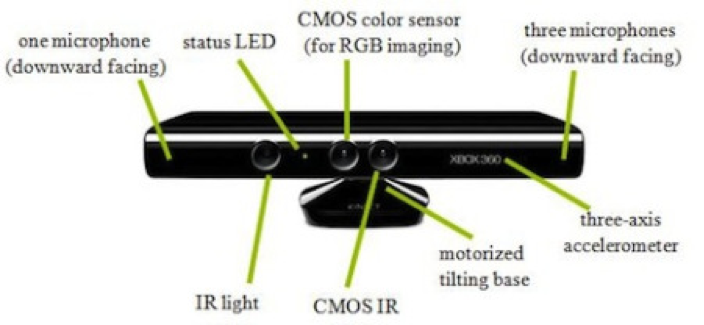
\includegraphics[width=1.0\textwidth]{images/kinect.png}
\label{fig:kinect}
\end{figure}

Because of its depth camera and infrared light emitor, the Kinect is able to provide a live depth map using a technique called structured light \cite{freedman_depth_2008}, which consists of projecting a known pattern of infrared dots into the scene and determine the depth by analyzing the pattern deformation. The kinect hardcodes all the information about the pattern (the dots and their relative distances) thus it can compare what it sees with what it stores and provide a live depth map of the scene (see Figure~\ref{fig:depthMap} \cite{lejeune_new_2011}).\\

\begin{figure}[h]
\caption{A depth map from the Kinect camera}
\centering
    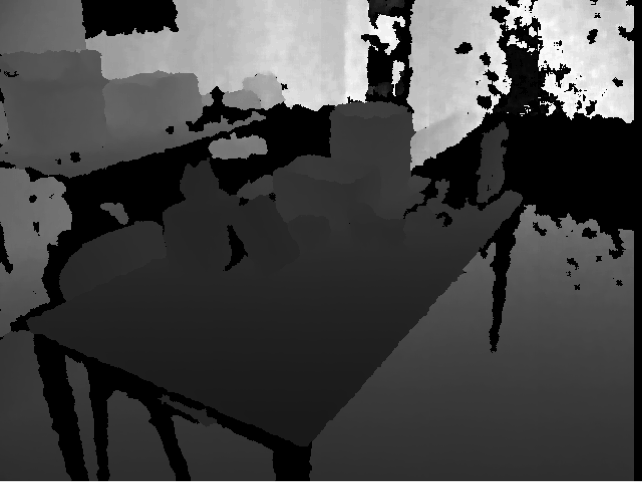
\includegraphics[width=0.7\textwidth]{images/depthMap.png}
\label{fig:depthMap}
\end{figure}

The Microsoft Kinect has the advantage to be relatively low cost and offers many useful API included the KinectFusion toolkit. KinectFusion provides fast 3D surface reconstruction by scanning the object with the Kinect camera only. In addition, KinectFusion is fast and takes care of low level problems such as camera calibration (see section~\ref{sec:3D cartography method}), camera pose, surface reconstruction\ldots \\

The researches about KinectFusion started in 2011 by Shahram Izadi et al. \cite{izadi_kinectfusion:_2011}. Explaining in details the implementation of KinectFusion is beyond the scope of this state of art and more details can be found in \cite{newcombe_kinectfusion:_2011} and \cite{izadi_kinectfusion:_2011}. However, an interesting problem is the camera pose problem. The camera pose problem consists of finding the camera position and orientation inside of a given coordinates system. In order to solve the camera six degrees of freedom (6DOF) pose, KinectFusion uses the iterative closest point (ICP) algorithm.\\

The ICP algorithm is an algorithm used to find the transformation that minimizes the distance between two sets of points. ICP is normally used to reconstruct 3D surfaces from different views of the same object. However, KinectFusion uses it to obtain a 6DOF transform that aligns the current points with the ones from the previous depth frame. This transform therefore gives the Kinect global camera pose. At the first frame the camera pose will be set as an identity matrix, at the next frames the ICP algorithm will give the transformation to apply to the camera pose matrix in order to get the new pose of the Kinect camera.\\

One of the key features of the KinectFusion algorithm is its parallel execution \cite{izadi_kinectfusion:_2011} on the GPU thus fast camera tracking and real-time 3D reconstruction can be obtained. In consequence of that, only compatible DirectX11 graphics cards can meet the requirement to run KinectFusion \cite{kinect}.\\

Using 3D surface reconstruction tools like the KinectFusion solves the problem of acquiring a 3D surface of the prototype to map the lymphatic system on it.  In addition, image fusion, camera calibration and 6DOF pose solutions are offered by the KinectFusion toolkit. However, the Kinect camera cannot be used alone to obtain information about the lymphatic system. Indeed, fluorochromes will emit infrared lights as well and even though those infrared lights will be in a different range of the ones emitted from the Kinect camera, they can perturb the collected data. Therefore, a separated infrared camera will be used (see Section~\ref{sec:Hamamatsu camera} for more details about it).

\section{3D mapping method}
\label{sec:3D cartography method}

The 3D mapping of the lymphatic system will be the most complex step of this Master Thesis. It will require solving the camera pose (see Section~\ref{sec:3D surface reconstruction}), camera calibration and image stitching problems. Fortunately, all these problems can be solved more easily by using the OpenCV (Open Source Computer Vision) library. \\

OpenCV is a free library used in computer vision and real-time applications. It is written in C++ and has C, python and java interfaces. In addition, OpenCV is cross-platform and provides more than 2500 optimized algorithms \cite{opencv} which can be used for camera tracking, face recognition, image stitching, augmented reality, etc.  \\

The following paragraphs will cover briefly how OpenCV can be used to solve the previous mentioned problems. A deeper explanation will be given afterwards when the project will start. \\

\subsection{Camera calibration}
\label{sec:camera calibration}

Before explaining what camera calibration is and how OpenCV does it, some explanations about basic camera functioning must be given. The figures and formulas in the following paragraphs come from the work of Bradski et al. (2008) \cite{bradski_learning_2008}, the reader is invited to consult their book for further information.\\

First of all, the simplest camera model is the pinhole camera, in which the light going through a small hole is projected in the opposite surface of that hole. See Figure~\ref{fig:pinhole} \cite[p. 372]{bradski_learning_2008}. $X$ is the length of the object, $x$ is the projected object image, $Z$ is the distance from the camera to the object and $f$ is the focal length, i.e. the distance where converging/diverging rays are in a focus point.\\

\begin{figure}[t]
\caption{The Pinhole camera model}
\centering
    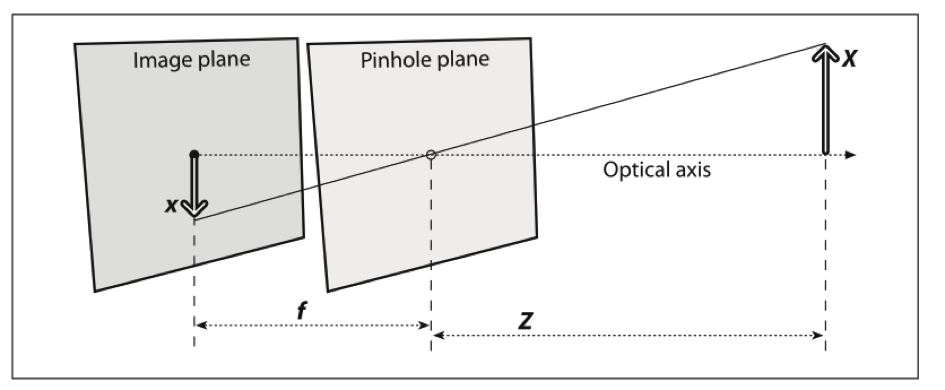
\includegraphics[width=1.0\textwidth]{images/pinhole.png}
\label{fig:pinhole}
\end{figure}

Like with the human eye, the projected image is inverted, which gives the following equation taken from \cite[p. 371]{bradski_learning_2008} (see the relationship between the two triangles):

\begin{equation}
  -x = f\frac{X}{Z}          
\end{equation}

Now, in order to eliminate the negative sign, the following model \cite[p. 372]{bradski_learning_2008} can be used instead of the one showed in Figure~\ref{fig:pinhole} (notice that the relationship between the two triangles is still valid):

\begin{figure}[h]
\caption{Simplified pinhole camera model}
\centering
    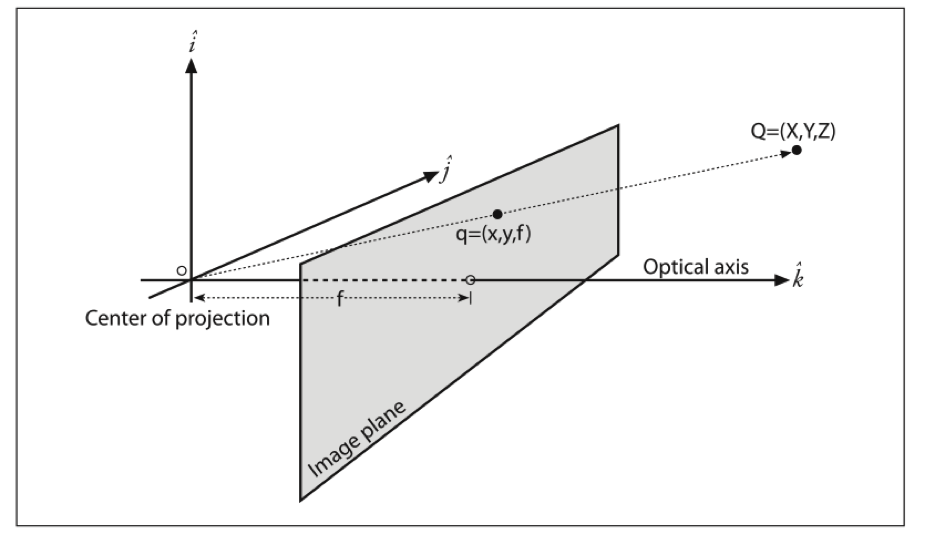
\includegraphics[width=1.0\textwidth]{images/simplifiedPinhole.png}
\label{fig:simplifiedPinhole}
\end{figure}

Next, two parameters $c_x$ and $c_y$ must be introduced. Indeed, one might think that the intersection of the projection center (see Figure~\ref{fig:simplifiedPinhole}) with the image plane is exactly at the center of the image plane. However, it is often not the case therefore these two parameters are used to adjust this displacement. The following formulas \cite[p. 373]{bradski_learning_2008} give the coordinates of a point in the image plane. 

\begin{equation}
  x = f_x\left(\frac{X}{Z}\right) + c_x \,\,\,\,\, y = f_y\left(\frac{Y}{Z}\right) + c_y    
\end{equation}

Finally, the following matrices \cite[p. 374]{bradski_learning_2008} give the transformation that maps a 3D point in the physical world to a 2D point in the image plane. $Q$ is a one-column matrix representing a 3D point in the physical world while $q$ represents the image plane point; $q$ is a 3 dimensions vector because homogeneous coordinates are used. $M$ is called the camera intrinsic matrix.

\begin{equation}\label{eq:q=MQ}
  q = MQ     
\end{equation}

\begin{equation}\label{eq:q=MQMatrice}
  q = \begin{bmatrix}
       u \\
       v \\
       w 
     \end{bmatrix}, 
  M = \begin{bmatrix}
       f_x & 0 & c_x \\
       0 & f_y & c_y \\
       0 & 0 & 1
     \end{bmatrix}, 
  Q = \begin{bmatrix}
       X \\
       Y \\
       Z 
     \end{bmatrix}     
\end{equation}

The pinhole camera model is simple but unfortunately the real cameras use lenses in order to gather more light. Lenses introduce some distortions, which have to be corrected. Two different distortions exist, radial distortions and tangential distortions \cite[p. 375]{bradski_learning_2008}. \\

Radial distortions can be corrected by the following formulas:
\begin{equation}
  x_{corrected} = x(1 + k_1r^2 + k_2r^4 + k_3r^6)    
\end{equation}
\begin{equation}
  y_{corrected} = y(1 + k_1r^2 + k_2r^4 + k_3r^6)    
\end{equation}
Tangential distortions can be corrected by the following formulas: 
\begin{equation}
  x_{corrected} = x + [2p_1y + p_2(r^2 + 2x^2)]    
\end{equation}
\begin{equation}
  y_{corrected} = y + [p_1(r^2 + 2y^2) + 2p_2x]
\end{equation}

Thus, in addition with the intrinsic matrix, a 5-by-1 matrix containing the $k_1$, $k_2$, $p_1$, $p_2$ and $k_3$ parameters has to be solved. Determining these two matrices is exactly what the calibration process is used for. \\

OpenCV uses the \textit{cvCalibrateCamera2()} function to do the calibration. The user has to target the camera to a known pattern/structure, usually a chessboard \cite{zhang_flexible_1999}. By taking multiple snapshots of the chessboard at different angles, OpenCV can determine the intrinsic parameters \cite{camera}. \\

In conclusion, camera calibration is used to correct distortions and obtain the different intrinsic parameters of the camera.

\subsection{Camera pose estimation}
\label{sec:Camera pose estimation}

As seen in the previous section, the equations~\ref{eq:q=MQ} and~\ref{eq:q=MQMatrice} provide a way to map a 3D point in the world to a 2D point in an image taken by a camera. However, those equations consider only the intrinsic camera parameters (the matrix $M$) and not the extrinsic parameters. A real camera is moving while recording multiple view of an object therefore the camera position is different at each frame. In consequence, for each frame, a transformation that determines the position of the camera has to be found. This transformation is a combination of a rotation and a translation matrix. \\

The equations becomes \cite{camera1}: 
\begin{equation}
  q = M\langle R\vert T\rangle Q     
\end{equation}
\begin{equation}
  q = \begin{bmatrix}
       u \\
       v \\
       w 
     \end{bmatrix}, 
  M = \begin{bmatrix}
       f_x & 0 & c_x \\
       0 & f_y & c_y \\
       0 & 0 & 1
     \end{bmatrix}, 
  \langle R\vert T\rangle =  \begin{bmatrix}
       r_{11} & r_{12} & r_{13} & t_1 \\
       r_{21} & r_{22} & r_{23} & t_2\\
       r_{31} & r_{32} & r_{33} & t_3
     \end{bmatrix},  
  Q = \begin{bmatrix}
       X \\
       Y \\
       Z 
     \end{bmatrix}     
\end{equation}

The matrix $M$ has to be computed only once but the transformation matrix $\langle R\vert T\rangle$ has to be computed every frame. In that purpose, some markers can eventually be placed inside the camera vision field (see Section~\ref{sec:proof of concept - introduction}). Those markers will be easily identifiable by the camera (usually a known pattern is used) therefore their position $q$ will be known. In addition, they will never change of position therefore the position $Q$ will also be known. Thus, determining the camera pose will only consist of solving a system of equations.

\subsection{Image stitching}

As mentioned before, because the camera does not have a wide field of vision, multiple overlapping images will have to be combined together to form only one. This process called image stitching can also be done with OpenCV.\\

One way OpenCV deals with it is by using SURF descriptors \cite{bay_surf:_2006} to find correspondences between two images targeting the same scene. Once the matching has been found, OpenCV finds the homography matrix to match the two images together. 

\section{Conclusion}

The lymphatic system plays an important role for the body. Obtaining structural information about it is an important task in the medical field. This state of art gave a brief overview of the different problems that can occur during this project. The remaining part of this Master Thesis will consist of building a working prototype for testing purposes, obtaining a 3D construction of it through a Kinect camera and finally, obtaining 3D information from NIR fluorochromes. In that purpose, the OpenCV library and its algorithms will be examined in more details.
